\section{Measured noise floor}
\label{app:floor}

Effect sizes in reward alignment are frequently comparable to run-to-run variation, so we
measured the variation rather than assuming it. We evaluated $8$ \emph{unmodified}
canonical arms -- differing only in training hardware (A100/H100/H200), world size ($3$ or
$4$), or random seed -- at the same outer epoch under the identical protocol, and formed
all $28$ pairwise differences of the reported composite.

\begin{center}
\begin{tabular}{lccc}
\toprule
& median $|\Delta|$ & mean $|\Delta|$ & max $|\Delta|$\\
\midrule
$28$ canonical-vs-canonical pairs & $0.39$ MDE & $0.46$ MDE & $1.23$ MDE\\
\bottomrule
\end{tabular}
\end{center}

Among pairs that match on \emph{all} of hardware, world size and seed -- i.e.\ pure
re-runs of the same configuration -- differences range from $0.06$ to $0.56$ MDE, the
latter with a per-image $t$ of $+1.95$. Per-image $t$ is computed over $1000$ images and
is therefore easy to make large; it does not measure run-to-run variation. We consequently
adopt the thresholds stated in Sec.~\ref{sec:exp:protocol}.

We also calibrated the two nuisance axes separately: changing world size from $3$ to $4$
on identical hardware is worth $+0.17$ MDE ($t=+0.58$), and the same canonical
configuration on H200/$4$ versus A100/$3$ differs by $0.07$--$0.54$ MDE across six
(checkpoint, prompt set, budget) cells, with $|t|<1.2$ in five of six. Cross-hardware
comparisons of two \emph{differences} therefore carry at most $\approx0.55$ MDE of slack.

The same arms also bound run-to-run variation on the \emph{absolute} scores, which is what
a reproduction claim rests on. Across seven unmodified canonical runs spanning three GPU
types, two world sizes and two random seeds, the full range of each reported column at
$100$ updates is:

\begin{center}
\begin{tabular}{lccccc}
\toprule
& Pick & CLIP & HPSv2.1 & Aes & ImgR\\
\midrule
median & $24.66$ & $0.316$ & $0.370$ & $5.90$ & $1.43$\\
full range & $0.02$ & $0.002$ & $0.001$ & $0.03$ & $0.02$\\
\bottomrule
\end{tabular}
\end{center}

Training is therefore reproducible at the absolute-score level to well under one part in a
hundred on every column; when we compare an absolute score against a published one, the
binding uncertainty is the evaluation pipeline (Sec.~\ref{sec:exp:repro}), not the training
run.

The headline \emph{difference} is similarly stable across independent training jobs. Our
$300$-update runs pass through $100$ updates on the way, so their checkpoints at that point
give a second, independently trained measurement of the same comparison at the same seed:
$+10.26$ versus $+10.70$ MDE at four steps and $+4.76$ versus $+5.62$ at forty on DrawBench,
differences of $0.44$ and $0.85$ MDE. Both sit inside the canonical-versus-canonical floor
measured above, and the run-to-run spread is \emph{smaller} than the seed-to-seed spread
($1.05$ MDE at four steps), which is the expected ordering.

\section{Held-out evaluator calibration}
\label{app:evalcal}

We required a held-out evaluator that actually tracks the quantity being optimized. Across
$12$ arms spanning $-35$ to $+18$ MDE on the reported composite, measured against a common
canonical baseline:

\begin{center}
\begin{tabular}{lcc}
\toprule
& $r$ with reported composite & sign agreement\\
\midrule
ImageReward & $\mathbf{+0.894}$ & $\mathbf{12/12}$\\
Aesthetic   & $-0.395$ & $4/12$\\
\bottomrule
\end{tabular}
\end{center}

Aesthetic is \emph{anti}-correlated and agrees in sign less often than chance; the most
extreme case is an arm at $-14.19$ MDE on the composite with Aesthetic $t=+27.70$. We
therefore report ImageReward as the held-out evaluator throughout and do not report
Aesthetic. We flag this because Aesthetic is commonly reported in this literature.

\section{Pairing requirements}
\label{app:pairing}

An arm and its baseline must match on training hardware, world size, random seed, and
outer epoch. Two concrete failures we encountered illustrate the need:
comparing an arm at $50$ updates against a baseline at $100$ updates produced a spurious
$-12.32$ MDE that is almost entirely the checkpoint difference; and comparing an arm to a
baseline trained on different hardware inflated a $+17.39$ MDE effect to $+18.34$ MDE.

\section{Sampling schedules and a degenerate query state}
\label{app:schedule}

The $\sigma$ schedules used, obtained from the model's own scheduler:
\begin{center}
\begin{tabular}{ll}
\toprule
$N$ & $\sigma_0,\dots,\sigma_N$\\
\midrule
$10$ & $1.000,\,0.960,\,0.913,\,0.858,\,0.790,\,0.707,\,0.602,\,0.465,\,\mathbf{0.278},\,0.009,\,0$\\
$6$  & $1.000,\,0.923,\,0.819,\,0.668,\,\mathbf{0.432},\,0.009,\,0$\\
$4$  & $1.000,\,0.858,\,\mathbf{0.602},\,0.009,\,0$\\
\bottomrule
\end{tabular}
\end{center}
Because the query is selected by $\argmin_j|\sigma_j-\sigma^\star|$
(Eq.~\eqref{eq:query}), shortening the rollout \emph{implicitly} moves the query: at
$N\!=\!6$ the selected state is $\sigma_q=0.432$.

At $N\!=\!4$ the selection is pathological. Since
$|0.602-0.278|=0.324>|0.009-0.278|=0.269$, the default request selects the near-clean
state $\sigma_q=0.00893$, where $y_0\approx z_q$ and target construction degenerates; the
resulting run peaks at update $15$ and then declines monotonically. A ``train at $4$
steps'' baseline must therefore pin $\sigma^\star$ explicitly to the schedule's
second-to-last non-degenerate state. \textbf{This is itself a finding: a $4$-step rollout
does not contain \opsd's design query state.}

\section{Training cost}
\label{app:cost}

Wall-clock per optimizer epoch over the full $100$-update run, on identical hardware and
world size:
\begin{center}
\begin{tabular}{llcc}
\toprule
hardware & configuration & min/epoch & relative\\
\midrule
\multirow{3}{*}{H200 $\times4$} & canonical & $2.79$ & $1.00\times$\\
 & $+$ \MSP ($|\mathcal K|=2$) & $3.36$ & $\mathbf{1.21\times}$\\
 & $+$ \MSP ($|\mathcal K|=3$) & $3.59$ & $1.28\times$\\
\midrule
\multirow{2}{*}{H100 $\times4$} & canonical & $2.77$ & $1.00\times$\\
 & $+$ \MSP ($|\mathcal K|=2$) & $3.39$ & $\mathbf{1.22\times}$\\
\midrule
H200 $\times4$ & $6$-step rollout & $2.54$ & $0.90\times$\\
\bottomrule
\end{tabular}
\end{center}
Each figure is the median per-epoch wall clock over a run's checkpoint timestamps, dropping
the first twenty epochs so that start-up is excluded. The two-state default costs
$1.21\times$ on H200 and $1.22\times$ on H100, measured on the joint and the reward-specific
objective respectively, so the figure is not specific to one accelerator or one reward. The
marginal cost of a third state is a further $+0.07\times$.

\section{Checkpoint independence}
\label{app:ckpt}

The few-step gain of propagation over canonical at $4$ sampling steps, as a function of
training checkpoint (paired, $n=1000$, MDE units). Every entry compares an arm against a
canonical baseline trained on the \emph{same} hardware and world size at the \emph{same}
checkpoint; cells without such a control are left blank rather than filled with a
cross-hardware comparison.
% 自动生成,勿手改。源:paper_figs/make_table_ckpt.py
\begin{center}
\resizebox{0.98\linewidth}{!}{%
\begin{tabular}{ll ccccc c ccccc}
\toprule
& & \multicolumn{5}{c}{\textbf{NFE}$=$\textbf{4}} & & \multicolumn{5}{c}{\textbf{NFE}$=$\textbf{40}} \\
\cmidrule(lr){3-7}\cmidrule(lr){9-13}
$\mathcal K$ & set & $20$ & $30$ & $50$ & $80$ & $100$ & & $20$ & $30$ & $50$ & $80$ & $100$\\
\midrule
$\mathcal K=\{3,6\}$ (default) & DrawBench & $+6.66$ & $+5.56$ & $+7.52$ & $+10.42$ & $+10.70$ & & $+2.39$ & $+3.44$ & $+3.19$ & $+5.27$ & $+5.62$ \\
 & Unseen-1k & $+5.95$ & $+4.83$ & $+6.06$ & $+8.19$ & $+8.20$ & & $+1.38$ & $+1.50$ & $+1.22$ & $+3.03$ & $+3.34$ \\
\addlinespace[2pt]
$\mathcal K=\{5,6,7\}$ & DrawBench & $+8.16$ & $+5.43$ & $+7.05$ & $+9.15$ & $+8.48$ & & -- & -- & $+1.46$ & -- & $+2.51$ \\
 & Unseen-1k & $+7.37$ & $+5.38$ & $+6.09$ & $+7.62$ & $+6.47$ & & -- & -- & $-0.15$ & -- & $+0.92$ \\
\addlinespace[2pt]
\bottomrule
\end{tabular}}
\end{center}

The dip at $30$ updates appears on \emph{both} prompt sets, so it is a property of the
training trajectory rather than evaluation noise. Every cell exceeds $+5.38$ MDE, so the
effect does not depend on stopping at $100$ updates.

\begin{figure}[h]
\centering
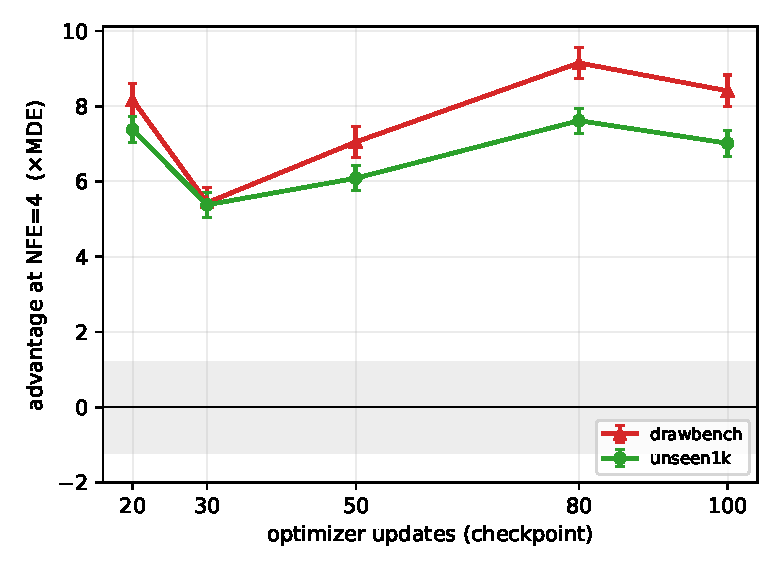
\includegraphics[width=0.78\linewidth]{fig4_advantage_vs_ckpt.pdf}
\caption{Few-step advantage of \MSP over canonical as a function of training checkpoint.
The effect is present from the earliest checkpoint we evaluate and does not depend on
stopping at $100$ updates.}
\label{fig:ckpt}
\end{figure}

\section{Training length: the gain at the published budget}
\label{app:budgetceiling}

Every other result in this paper is measured at $100$ updates. To follow the comparison to
the published $300$ we trained two independent pairs of runs, each pair a propagation run and
a canonical run with the same seed on the same node and world size, and evaluated both members
of a pair at the same five checkpoints. The second pair was pre-registered as a replicate after
the first showed a late collapse.

\begin{figure}[h]
\centering
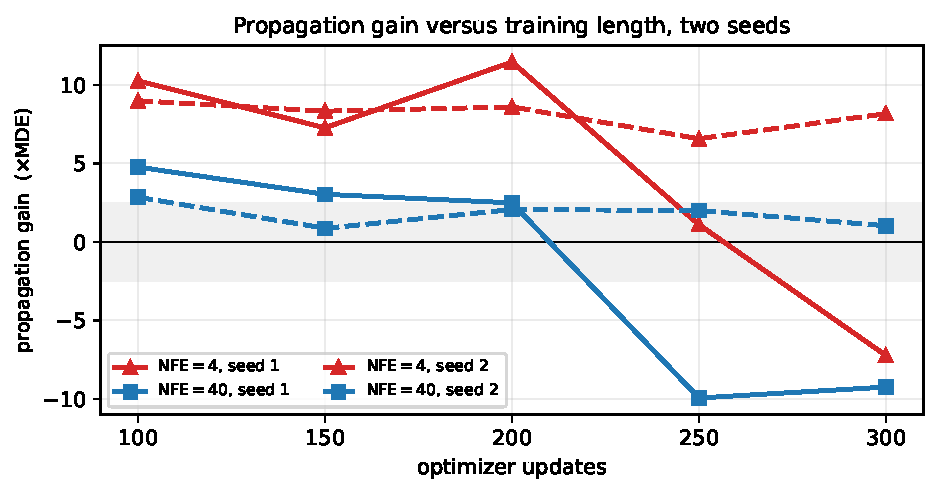
\includegraphics[width=0.74\linewidth]{fig11_gain_vs_updates.pdf}
\caption{\textbf{Propagation gain versus training length}, DrawBench, for two independent
pairs of $300$-update runs (solid: seed 1, dashed: seed 2); each point pairs the two runs of
one seed at the same checkpoint. Shaded: $\pm2.5$ MDE, the band a single seed cannot resolve.
At four steps seed 1 peaks at $200$ updates ($+11.46$) and is $-7.23$ by $300$, while seed 2
stays between $+6.57$ and $+8.99$ at every checkpoint. At forty steps neither seed is above
the band at $300$ updates.}
\label{fig:budgetceiling}
\end{figure}

The two seeds disagree about what happens after $200$ updates and agree about forty steps.
At four steps seed 2 keeps a significant lead at every checkpoint ($+8.99$, $+8.32$, $+8.60$,
$+6.57$ and $+8.16$ MDE on DrawBench, $+3.55$ to $+7.72$ on Unseen-1k, every cell $t\ge8.8$),
whereas seed 1 collapses from $+11.46$ at $200$ updates to $-7.23$ at $300$. At forty steps
the seed-2 gain is small throughout ($+0.86$ to $+2.84$ on DrawBench, $+0.03$ to $+1.71$ on
Unseen-1k) and at $300$ updates is $+1.02$ / $+0.24$ MDE, a tie by our threshold; seed 1 is
$-9.25$ / $-14.28$. So the late collapse is something a run \emph{can} do rather than something
it reliably does --- one run of two --- and neither seed supports a forty-step gain at the
published budget. We report the seeds side by side rather than averaged: at $300$ updates an
average would be dominated by the seed-1 collapse and would describe neither run.

The rest of this section concerns the seed-1 collapse. Two readings are consistent with it and
we cannot separate them. The training reward of the propagation arm peaks higher than the canonical arm's ($1.7051$ versus $1.6626$, both
near epoch $227$) and then falls back to $94.5\%$ of its own peak while the canonical arm
holds $97.8\%$, so the collapse is visible in the training objective as well as in the
evaluation.

Two further measurements bear on which reading is right, and both point away from the
extra states. First, \emph{the collapse does not recur} in the independent seed-2 pair above, nor in a
run that resumes the seed-1 propagation arm from its own $200$-update checkpoint and continues
with propagation still on: over updates $250$ to $300$ that run \emph{gains} $3.80$ MDE at four
steps on DrawBench while the continuous run loses $5.93$. Second, it is not an evaluation artifact: averaging the weights of checkpoints
$280$, $290$ and $300$ leaves the gap to canonical unchanged ($-7.23$ to $-7.45$ MDE at
four steps, and $-11.81$ to $-11.93$ on Unseen-1k), so a single noisy checkpoint is not what
produces it. Taken together the collapse looks like an optimisation-trajectory event rather
than a property of propagating to extra states.

The seed-2 pair is the clean replicate that the resumed arm could not be: resuming by itself
moves the score a great deal in this setting ($+16.11$ MDE at four steps against the continuous
arm at $300$ updates), so on its own the resumed arm could have been masking the collapse rather
than showing it was never there. With both, we read the collapse as a risk rather than a ceiling:
it happened in one of two independent runs, and two runs are too few to estimate how often.

That last perturbation turns out to be informative in its own right, because it is not generic.
Applying the same restart to the \emph{canonical} arm --- resuming it from its own $200$-update
checkpoint and continuing canonically to $300$ --- moves its score by $-0.38$ and $-0.03$ MDE on
DrawBench at four and forty steps and by $-0.06$ and $-0.32$ on Unseen-1k, four cells all inside
the $1$ MDE band we treat as no effect ($|t|\le1.65$). The same perturbation on the propagation
side is $+16.11$ and $+11.56$ on DrawBench and $+19.08$ and $+15.27$ on Unseen-1k. A restart is
therefore not an evaluation perturbation that any run of this kind would respond to; it is
specific to weights trained with propagation. The only discontinuity a resume introduces is that
the live parameters are replaced by their own exponential moving average, since checkpoints are
written from the EMA while the optimiser, EMA buffer and RNG states are all restored --- so what
a restart changes is the point the last $100$ updates start from, not the parameters that get
evaluated. Averaging final parameters after the fact does not reproduce the effect on either
side: souping checkpoints $280$, $290$ and $300$ moves the propagation arm by $-0.49$ to $-1.70$
MDE and the canonical arm by $-0.01$ to $-0.45$ across the same four cells. Why the propagation
arm's live parameters sit somewhere from which a further $100$ updates end up so much worse than
from their own average, we have not measured. What we can say is that the seed-1 collapse is not robust to a perturbation as small as
restarting the same run from its own checkpoint. Whether it is over-optimisation specific to the extra states, or a generic
late-training instability that propagation reaches sooner because it optimises faster, is not
something these runs can decide.

For the seed-1 pair one practical consequence is worth stating plainly. If propagation is stopped at $200$
updates --- two thirds of the published training cost --- it is still $+6.10$ MDE ahead of
the canonical run trained for the full $300$ at four steps, though $-2.63$ behind it at
forty. Spending the remaining third on the canonical objective instead of stopping removes
that forty-step deficit: a run that propagates for $200$ updates and then continues
canonically to $300$ is $+11.44$ / $+9.66$ MDE ahead at four steps and $+5.65$ / $+4.64$ ahead
at forty (DrawBench / Unseen-1k), measured against a canonical run that was itself restarted at
$200$ updates so that the restart discussed above is present on both sides.

We do not read that as a gain from switching objectives. The switch measured on its own ---
against the same restarted propagation run continued with propagation still on --- is $+2.19$
/ $+2.33$ MDE at four steps, below the $2.5$ MDE threshold a single seed has to clear
elsewhere in this paper, and its share of the total fell from $34.1\%$ / $30.4\%$ at $250$
updates to $19.1\%$ / $24.1\%$ at $300$. The larger part of the difference is carried by the
restart effect above, which we do not understand. This is one seed, we did not pre-register an
early-stopping rule, have no held-out split for choosing a checkpoint, and chose the switch
point after seeing where the gain peaked --- so we report the whole of it as an observation
about these runs rather than as a schedule we would recommend.

\section{Which states to propagate to}
\label{app:family}

Our default $\mathcal K=\{3,6\}$ ($\sigma=0.858,\,0.602$) reaches higher noise than the
alternative $\mathcal K=\{5,6,7\}$ ($\sigma=0.707,\,0.602,\,0.465$), which uses \emph{more}
states but tops out at $\sigma=0.707$. At the main checkpoint ($100$ updates) and against
the same control (paired gain in MDE, DrawBench / Unseen-1k):

\begin{center}
\resizebox{0.98\linewidth}{!}{%
\begin{tabular}{lcccccc}
\toprule
$\mathcal K$ & NFE$=2$ & $4$ & $6$ & $10$ & $20$ & $40$\\
\midrule
$\{3,6\}$ (ours) & $+15.3$ / $+16.4$ & $+10.7$ / $+8.2$ & $+7.1$ / $+4.6$ & $+5.8$ / $+3.8$ & $+5.5$ / $+3.4$ & $+5.6$ / $+3.3$\\
$\{5,6,7\}$      & $+20.1$ / $+21.1$ & $+8.5$ / $+6.5$ & $+4.3$ / $+2.7$ & $+2.5$ / $+1.3$ & $+2.0$ / $+0.8$ & $+2.5$ / $+0.9$\\
\bottomrule
\end{tabular}}
\end{center}

One caveat on that table. The $\{5,6,7\}$ arm was trained on a different node type and world
size from everything else here ($3\times$A100 rather than $4\times$H200), so pairing it against
the $4$-GPU control crosses two axes at once. We checked that the conclusion does not depend
on which control we use: against the matched-world-size control instead, its four-step gain is
$+8.04$ / $+6.77$ rather than $+8.48$ / $+6.47$, so the default still leads by $2.2$--$2.7$ MDE
either way. We report the $4$-GPU control in the table because every other row uses it.

Adding a third state does not help, and neither does reaching higher noise. A third
member, $\mathcal K=\{2,3,4\}$ ($\sigma$ up to $0.913$), was trained under the same
protocol. At $100$ updates the default beats it in all four cells -- $-1.30$ and $-1.91$
MDE on DrawBench, $-3.24$ and $-2.63$ on Unseen-1k at $4$ and $40$ steps, the last two
clearing the significance threshold against it. That ordering is not stable across
checkpoints: at $50$ updates the higher set is ahead on DrawBench at four steps
($-1.74$ MDE for the default), so the interior optimum is a statement about the main
checkpoint, not about every point along training. Against the canonical baseline the three
members order as $+10.70/+8.20$ (default), $+9.40/+4.96$ (higher), $+8.48/+6.47$ (lower)
at $4$ steps and $+5.62/+3.34$, $+3.70/+0.70$, $+2.51/+0.92$ at $40$: the default is best
in every cell. The supervision set therefore has an \emph{interior} optimum in the noise
level it reaches, near $\sigma\!\approx\!0.858$.
From $4$ steps upward the two-state set that reaches $\sigma=0.858$ is ahead of the lower
set on both prompt sets, by $+1.7$ to $+3.5$ MDE ($+2.2$ to $+3.5$ on DrawBench, $+1.7$ to
$+2.6$ on the held-out set), and the gap widens with the budget; the lower set decays toward the measured floor while ours flattens at a
positive value (Fig.~\ref{fig:family}). The one exception is $2$ steps, where the lower
set is ahead by about $4.7$ MDE -- at that budget the sampling grid has no interior state
at all ($\sigma\in\{1.000,\,0.009,\,0\}$), so the design principle has nothing to match.

\begin{figure}[h]
\centering
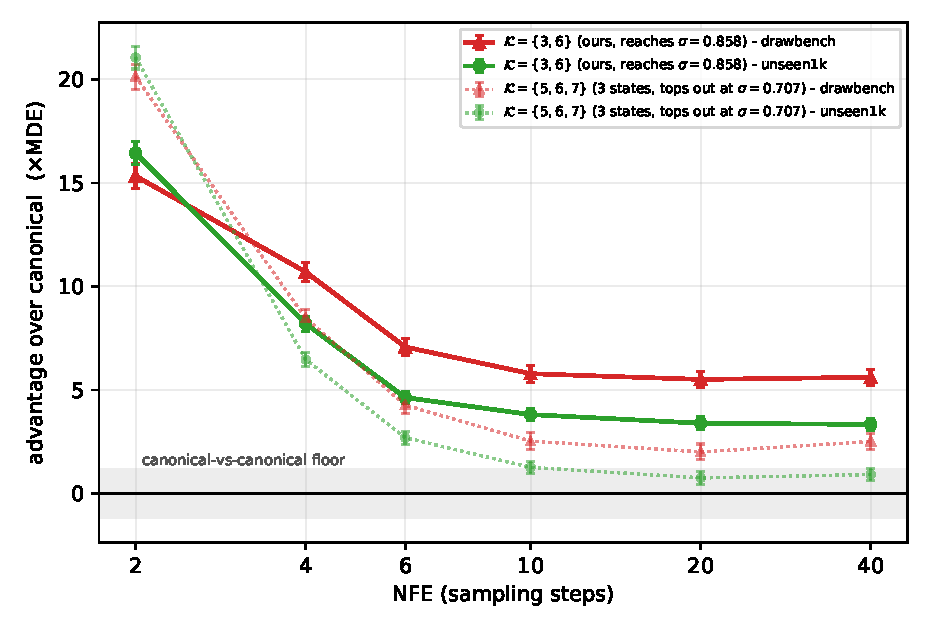
\includegraphics[width=0.78\linewidth]{fig3_advantage_vs_nfe.pdf}
\caption{Advantage over canonical for two members of the propagation family at $100$
updates. Solid: $\mathcal K=\{3,6\}$, which reaches $\sigma=0.858$. Dotted:
$\mathcal K=\{5,6,7\}$, which uses three states but tops out at $\sigma=0.707$. Shaded band
is the measured canonical-versus-canonical floor. The lower set decays toward the floor;
ours flattens at a positive value.}
\label{fig:family}
\end{figure}

\section{Per-axis results}
\label{app:peraxis}

Paired $t$ per reward axis, \MSP versus canonical at $100$ updates:
% 自动生成,勿手改。源:paper_figs/make_table_peraxis.py
\begin{center}
\small
\begin{tabular}{llcccccc}
\toprule
set & axis & NFE$=2$ & $4$ & $6$ & $10$ & $20$ & $40$\\
\midrule
\multirow{4}{*}{DrawBench}
 & PickScore    & $+17.81$ & $+15.71$ & $+12.35$ & $+10.30$ & $+10.80$ & $+11.04$\\
 & CLIP         & $+14.76$ & $+14.32$ & $+10.70$ & $+9.08$ & $+9.22$ & $+9.40$\\
 & HPSv2        & $+34.83$ & $+24.62$ & $+18.48$ & $+14.66$ & $+13.41$ & $+12.89$\\
 & ImageReward  & $+15.14$ & $+11.24$ & $+9.02$ & $+8.32$ & $+7.63$ & $+7.88$\\
\midrule
\multirow{4}{*}{Unseen-1k}
 & PickScore    & $+18.37$ & $+18.09$ & $+11.85$ & $+9.81$ & $+9.66$ & $+10.13$\\
 & CLIP         & $+16.61$ & $+10.01$ & $+7.51$ & $+6.88$ & $+5.99$ & $+5.98$\\
 & HPSv2        & $+40.81$ & $+24.78$ & $+15.98$ & $+10.73$ & $+8.14$ & $+7.42$\\
 & ImageReward  & $+21.50$ & $+9.95$ & $+6.25$ & $+4.35$ & $+1.50$ & $+1.18$\\
\bottomrule
\end{tabular}
\end{center}


\begin{figure}[h]
\centering
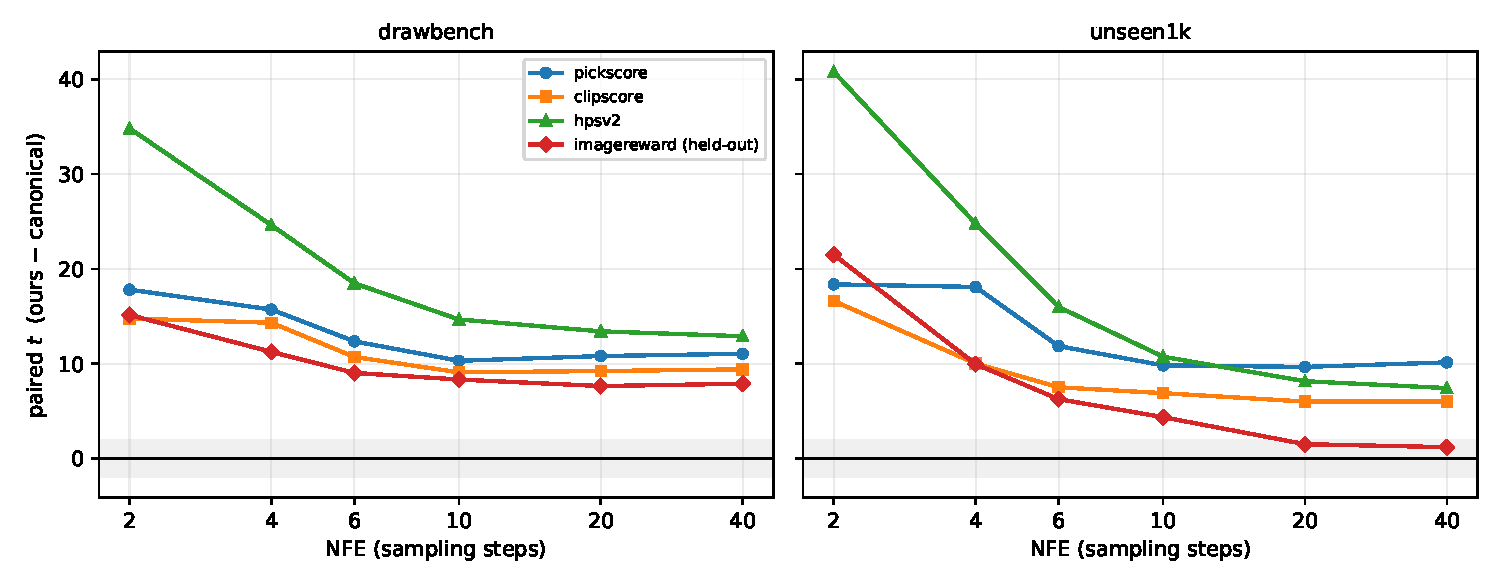
\includegraphics[width=\linewidth]{fig5_peraxis_vs_nfe.pdf}
\caption{Per-axis paired $t$ versus sampling budget. Every axis moves in the same
direction at every budget; the gain is not carried by one reward component.}
\label{fig:peraxis}
\end{figure}

\section{Extreme budget}
\label{app:flow2}

At $2$ sampling steps both models are far outside their usable range -- canonical falls to
a composite of $1.10$, below the \emph{untrained} model at $4$ steps ($1.11$) -- but the
relative ordering is preserved and the gap widens: \MSP is $+15.33$ MDE on DrawBench
($80.2\%$ win rate) and $+16.44$ on Unseen-1k ($84.6\%$). We report this for completeness;
we do not claim $2$-step generation is practical here.

\section{Unselected qualitative samples}
\label{app:qual}

Figure~\ref{fig:qual} selects prompts by a rule fixed in advance: among prompts where our
model's absolute score is above the median, the ones with the largest paired improvement.
For completeness Fig.~\ref{fig:qualunsel} shows a panel drawn without any selection -- the
first eight prompts of the evaluation file in file order.

Those unselected prompts are dominated by DrawBench's adversarial text-rendering and
counting categories. It would be easy to assume that nothing can be seen there because the
model cannot render them; that assumption is wrong. Ranked by paired improvement at four
steps, those same categories are where propagation helps \emph{most}: the twelve
largest-gain prompts are all of this kind, with gains of $+0.18$ to $+0.26$ composite
against a dataset mean of $+0.035$. What makes them poor figure material is their low
\emph{absolute} score, not an absence of difference, which is why the selection rule
conditions on absolute score and then ranks by improvement.

\begin{figure}[h]
\centering

\includegraphics[width=\linewidth]{fig8_qual_unselected.pdf}
\caption{Unselected panel: the first eight evaluation prompts in file order, four sampling
steps, rendered at the same display setting as Fig.~\ref{fig:qual} (guidance $1.5$) so that
the only difference between the two panels is whether the prompts were selected.}
\label{fig:qualunsel}
\end{figure}

\section{The evaluation protocol is not a display protocol}
\label{app:protocol}

Every number in this paper uses the protocol inherited from prior work: $512\times512$,
classifier-free guidance disabled, and the stated number of sampling steps. That protocol
is the right one for \emph{comparison} -- all arms share it and all comparisons are paired
-- but it is a poor setting for \emph{looking at} images, and it also exaggerates one
specific defect.

\paragraph{A frequency measurement.} Reward-trained SD3.5-M checkpoints carry a periodic
texture at the VAE stride ($8$ px) and the patch stride ($16$ px). We quantify it as the
ratio of the spectral magnitude at that period to a local baseline, averaged over the two
image axes; $1.0$ means no periodic structure. The untrained base model scores $1.27$
under the evaluation protocol and $1.03$ once guidance and $40$ steps are restored, so the
structure is not an artifact of the architecture. Reward training raises it: our canonical
reproduction reaches $2.29$ and \MSP $2.57$, while the publicly released single-reward
OPSD checkpoints sit at $1.51$ and $1.56$. Restoring guidance and steps lowers all of them
-- canonical to $1.48$, \MSP to $1.71$, the released checkpoint to $1.22$ -- while the
reported composite \emph{rises} ($1.5460\!\to\!1.6373$ for canonical). The protocol
therefore inflates the defect by roughly $1.5\times$ on top of whatever training produces.

\paragraph{Resolution is not the cause.} At matched guidance and steps, $1024$ and $512$
are indistinguishable ($1.4709$ vs.\ $1.4639$ composite, $1.02$ vs.\ $1.03$ texture).
Removing guidance at $1024$ costs more than halving the resolution does ($1.2380$).

\paragraph{No scalar evaluator sees it.} The texture grows monotonically with training
($1.18$ at $20$ updates to $2.29$ at $100$) while both the reported composite and the
held-out ImageReward improve monotonically over the same range. A frequency measurement is
therefore not redundant with the reward scores; it is the only instrument here that
registers this particular failure.

\paragraph{Choosing a display setting.} Guidance also has an optimum at four steps. Scaling
it from $1.0$ to $4.5$ drives the fraction of pixels clipped to $0$ or $255$ from
$0.4\%$ to $42.8\%$ (canonical) and the composite from $1.5460$ down to $1.3144$. Guidance
$1.5$ maximises the composite ($1.5861$) at $2.6\%$ clipped pixels, and we use it for the
qualitative panels only.

\begin{figure}[h]
\centering
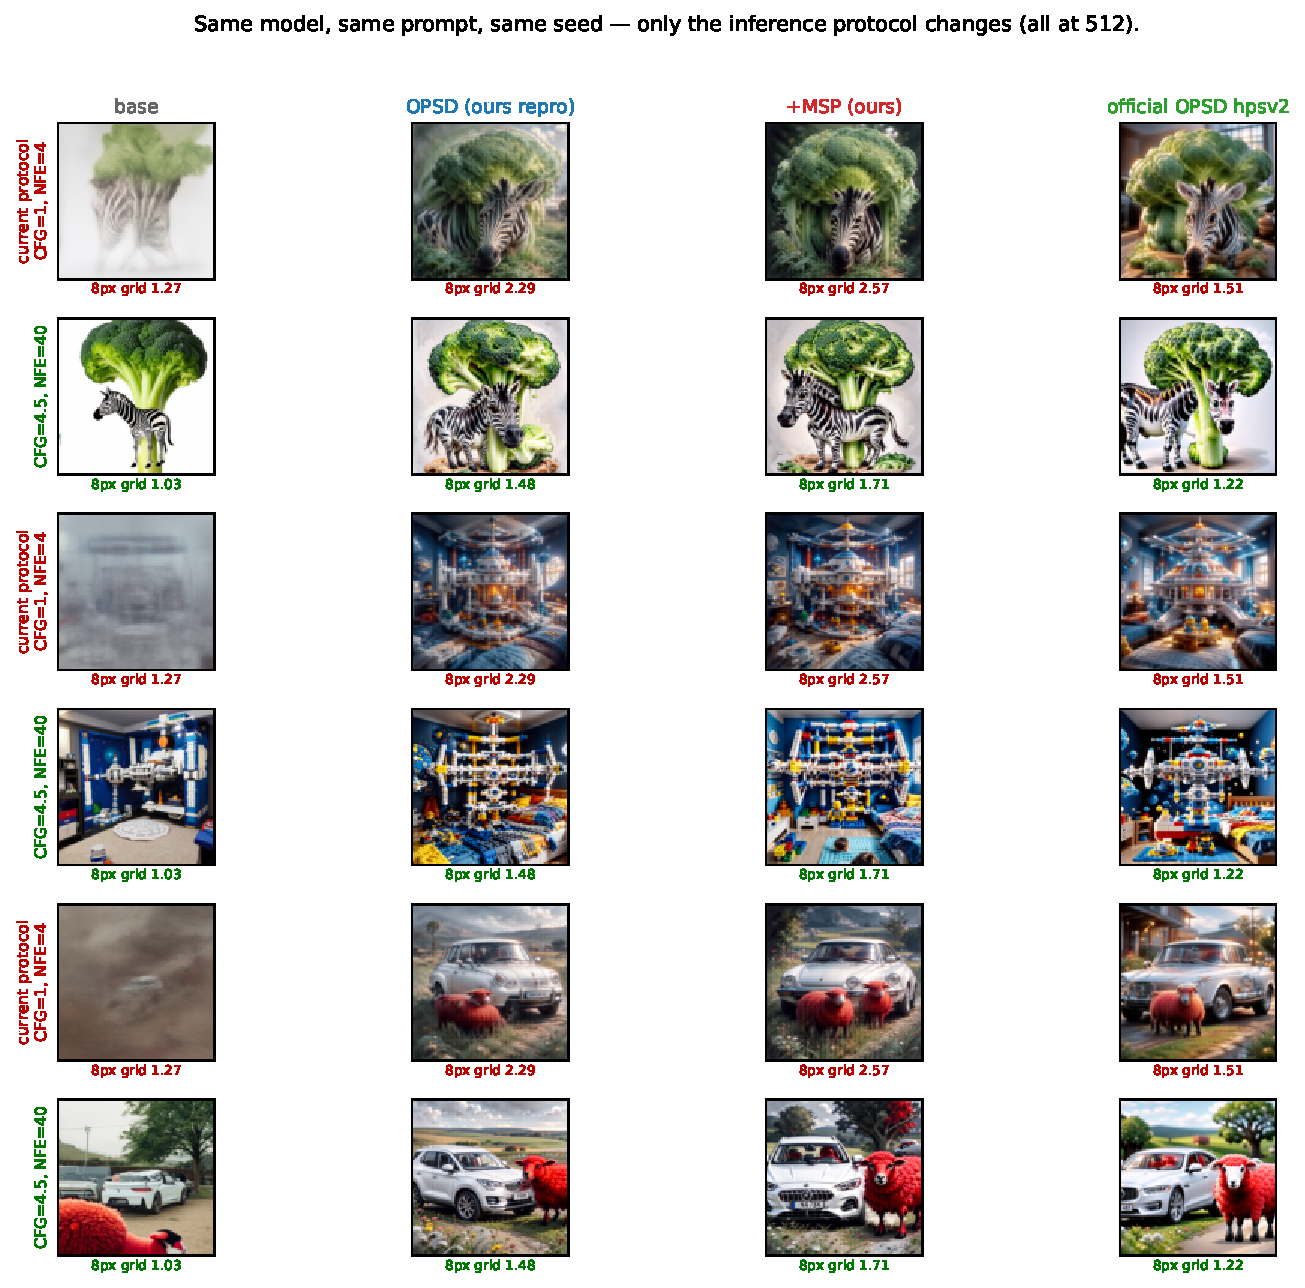
\includegraphics[width=\linewidth]{fig9_protocol_cmp.pdf}
\caption{\textbf{The high-frequency texture is a property of the display protocol, not of
our method.} Same prompts, same seed, $512^2$; only the inference protocol changes between
the two rows of each pair. Numbers are the $8$-pixel (VAE stride) spectral peak divided by
its local baseline; $1.0$ means no periodic structure. Under the evaluation protocol
(CFG-free, four steps) every reward-trained checkpoint is elevated -- including the
\emph{published} \opsd{} checkpoint at $1.51$ -- while the untrained backbone sits at
$1.27$. Raising guidance and the step count brings all four columns down. No scalar
evaluator in this literature detects this; only the spectrum does.}
\label{fig:protocolcmp}
\end{figure}

\section{Does the gain survive on a stronger baseline?}
\label{app:stack}

A method that only helps a weak baseline is fragile. We therefore stack propagation on the
strongest single-arm configuration in our study: a learning-rate variant that reaches
$+17.95$ MDE over canonical at the full budget and $+18.86$ at four steps -- that is, a
baseline whose advantage is essentially flat in the sampling budget (the difference between
the two, $+0.91$ MDE, is the quantity we care about).

Propagating on top of it, at a matched checkpoint, matched hardware and matched seed, and
comparing the two directly rather than through a shared control:

\begin{center}
\begin{tabular}{lcccc}
\toprule
& \multicolumn{2}{c}{\textbf{DrawBench}} & \multicolumn{2}{c}{\textbf{Unseen-1k}}\\
\cmidrule(lr){2-3}\cmidrule(lr){4-5}
& NFE$=4$ & NFE$=40$ & NFE$=4$ & NFE$=40$\\
\midrule
gain over the strong baseline, $50$ updates & $+6.00$ & $+2.40$ & $+4.79$ & $+0.03$\\
gain over the strong baseline, $100$ updates & $+2.95$ & $-3.53$ & $+3.01$ & $-4.68$\\
\bottomrule
\end{tabular}
\end{center}

The budget-dependent part -- the four-step value minus the full-budget value -- is $+3.60$
and $+4.76$ MDE at $50$ updates and $+6.48$ and $+7.70$ at $100$. Propagation on its own
produces $+5.59$ on the same quantity and the learning-rate baseline alone produces
$+0.91$, so the budget-dependence is supplied by the propagation rather than by the
stronger optimisation, and it survives stacking at both checkpoints.

The absolute picture changes between the two checkpoints, and we report it rather than
only the criterion. At $50$ updates stacking is a uniform improvement over the strong
baseline. By $100$ updates it has become a trade: still ahead at four steps, but
$3.5$--$4.7$ MDE behind at the full budget. In this respect the stacked configuration
behaves like the (A$+$C) and (B$+$C) combinations of Sec.~\ref{sec:exp:compose} rather than
like pure propagation, which does not trade.

One caveat: this arm uses the lower supervision set $\mathcal K=\{5,6,7\}$ rather than the
default $\{3,6\}$, because it was launched before the family comparison in
App.~\ref{app:family} settled. The default is better than this member in every cell there,
so the stacking result is a lower bound on what the default would give; we have not run the
default in the stacked configuration and do not report it as if we had.

\section{Reward-specific checkpoints}
\label{app:rewardspec}

The published main table has a second block in which each column is filled by the
checkpoint trained on \emph{that} evaluator, at $100$ optimizer updates and branch
coefficient $\beta=1.0$. We reproduce that block and add propagation to it, under the same
protocol and the same per-reward convention.

% 自动生成,勿手改。源:paper_figs/make_table_rewardspec.py
\begin{center}
\begin{tabular}{l rrr}
\toprule
\textbf{Model} & \textbf{HPSv2.1} & \textbf{Pick} & \textbf{CLIP}\\
\multicolumn{4}{l}{\footnotesize each column is filled by the checkpoint trained on that evaluator}\\
\midrule
SD3.5-M w/o CFG & $0.207$ & $20.59$ & $0.241$\\
$+$ \opsd (reward-specific) & $0.392$ & $24.96$ & $0.320$\\
$+$ \MSP (reward-specific) & $0.391$ & $24.95$ & $0.319$\\
\bottomrule
\end{tabular}
\end{center}


For reference, the published reward-specific row reports HPSv2.1 $0.390$, PickScore
$24.94$ and CLIPScore $0.340$. Cells that are not yet filled are left blank; no number is
borrowed across rewards.

\paragraph{Reproduction.}
Our reward-specific canonical run reaches HPSv2.1 $0.392$ against the published $0.390$ --
a $0.5\%$ agreement, obtained with no tuning beyond matching the stated protocol. Together
with the joint-objective parity of Sec.~\ref{sec:exp:repro} this establishes that the
baseline we improve upon is the published method, not a weakened variant of it.

\paragraph{Every reward-specific run, on the same thresholds.}
Each row compares propagation against the canonical run trained on the \emph{same} single
reward, scored on that reward, at the published $100$-update budget. The verdict column
applies the thresholds fixed in advance (Sec.~\ref{sec:exp:protocol}): $+$ significant gain,
$0$ no effect, $-$ significant loss. The deficit ratio is each model's own four-step deficit
for \MSP divided by the canonical one, as in the table above.

% 自动生成,勿手改。源:paper_figs/make_table_rsverdict.py
\begin{center}
\begin{tabular}{lcccccc}
\toprule
& \multicolumn{2}{c}{NFE$=4$ (paired $t$)} & \multicolumn{2}{c}{NFE$=40$} & &\\
\cmidrule(lr){2-3}\cmidrule(lr){4-5}
\textbf{training reward} & DrawB. & Uns.-1k & DrawB. & Uns.-1k & deficit ratio & verdict\\
\midrule
HPSv2.1 & $+0.27$ & $-0.31$ & $-1.22$ & $-3.67$ & $0.97$\,/\,$0.95$ & $0$\\
PickScore & $-15.68$ & $-14.12$ & $-0.42$ & $-3.09$ & $1.70$\,/\,$1.58$ & $-$\\
CLIPScore & $+5.15$ & $+4.80$ & $-2.30$ & $-2.59$ & $0.48$\,/\,$0.46$ & $0$\\
ImageReward & $+12.11$ & $+7.92$ & $+4.41$ & $+3.52$ & $0.35$\,/\,$0.47$ & +\\
Aesthetic & $-274.71$ & $-292.47$ & $-140.82$ & $-158.02$ & $3.81$\,/\,$4.19$ & n/a$^{\dagger}$\\
\bottomrule
\end{tabular}
\\[2pt]{\footnotesize $^{\dagger}$No verdict: both arms of this pair score \emph{below the untrained}
base model on the reported composite in all four cells, so the comparison is between two
collapsed models and does not measure few-step quality. Numbers are shown unchanged.}
\end{center}


The objectives do not agree with each other --- the four that yield a verdict span a
significant loss, two null results and a significant gain --- which is why the
pre-registration fixed that all of them be reported rather than summarised into one
number.

\paragraph{The reward-specific outcome depends on the reward.}
Propagation is harmful at four steps on PickScore, neutral on HPSv2.1 and on CLIPScore, and
helpful on ImageReward. The fifth recipe, Aesthetic, yields no verdict, for a reason that is
about the recipe and not about propagation: \emph{both} arms end up below the untrained base
model on the reported composite in all four cells ($0.93$--$1.00$ against $1.07$--$1.24$) while
the Aesthetic score they are trained on more than doubles ($4.7$--$5.6$ to $10.2$--$12.2$), and
the gap to the base model widens with further training. Comparing two collapsed models on the
score they are both exploiting does not measure few-step quality, so we report the numbers and
withhold the verdict. On that score propagation is far behind ($t=-46$ at four steps); we state
it rather than omit it, but it is not evidence about the method.

This is a property of the published recipe, not of our run, and the reproduction is what shows
it. The published reward-specific Aesthetic figure is $12.08$ (and $12.09$ for ReFL, $9.11$ for
DiffusionNFT, against $5.12$ for the untrained backbone), and our canonical Aesthetic run
reaches $12.18$ --- a $0.87\%$ difference, inside the $1.6\%$ tolerance of
App.~\ref{app:protocol}. That same checkpoint sits below the untrained backbone on
\emph{all five} other evaluators: composite $0.943$ vs.\ $1.240$, ImageReward $-1.58$ vs.\
$-0.55$, PickScore $17.81$ vs.\ $20.59$, CLIPScore $0.068$ vs.\ $0.241$, HPSv2.1 $0.189$ vs.\
$0.207$. We reproduce the published number closely and report what it costs; we draw no
comparison of methods from it.

There is a second reason this pair is not a comparison, and it is about our run rather than the
recipe: the \MSP arm \emph{diverged}. Its training reward rises normally to $10.34$ at update
$42$, then falls to $4.90$ by update $56$ --- below the $5.75$ it started from, for seven
consecutive updates --- and recovers only to $7.09$ by update $100$, never regaining the peak.
The canonical arm rises over the same range with no comparable event: it never falls below
its own starting value, and its largest drawdown from its running peak is small enough that the
same check does not flag it. At update $100$ the \MSP arm scores
$4.42$ on the objective it was trained to maximise, below the $4.73$ of the untrained backbone.
We state this plainly: propagation was unstable under this recipe. We do not call it a
mechanistic failure of the method, because the instability occurs inside a regime where
\emph{both} arms are worse than no training at all, and we cannot separate ``propagation is
unstable on this objective'' from ``this objective is not trainable''. None of the four
reward-specific pairs that do yield verdicts triggers the same divergence check. This is a second and
independent reason to set Aesthetic aside: App.~\ref{app:evalcal} already shows it is a poor
\emph{yardstick} (anti-correlated with the composite), and this shows it is a poor
\emph{objective}. At the main checkpoint, paired over
$n=1000$ images, on each run's own training reward:

\begin{center}
\begin{tabular}{llccc}
\toprule
prompt set & NFE & \MSP & canonical & paired $t$\\
\midrule
\multirow{2}{*}{DrawBench} & $4$  & $0.3727$ & $0.3725$ & $+0.27$\\
                           & $40$ & $0.3915$ & $0.3920$ & $-1.22$\\
\midrule
\multirow{2}{*}{Unseen-1k} & $4$  & $0.4020$ & $0.4021$ & $-0.31$\\
                           & $40$ & $0.4211$ & $0.4223$ & $-3.67$\\
\bottomrule
\end{tabular}
\end{center}

At the budget where propagation delivers its largest joint-objective gain -- $4$ steps --
the two HPSv2 runs are indistinguishable on both prompt sets ($|t|<0.4$, win rate
$50$--$52\%$). Expressed against the canonical few-step deficit that propagation is designed
to close ($0.0195$ and $0.0201$ HPSv2.1 on the two sets), the change is $+0.7\%$ and
$-0.7\%$: zero to the precision of the measurement.

PickScore is worse than neutral. Trained on PickScore alone, propagation loses $0.58$ and
$0.51$ PickScore at four steps ($t=-15.68$ and $-14.12$, win rates $36\%$ and $38\%$) while
matching the canonical run at forty ($t=-0.42$ and $-3.09$); held-out ImageReward moves the
same way at four steps ($t=-7.57$ and $-3.89$), so this is not an artifact of the PickScore
evaluator. The signature is the inverse of the joint-objective one: measured against itself,
the canonical PickScore run has a four-step deficit of $0.82$ and $0.78$, and propagation
\emph{widens} it to $1.39$ and $1.23$ -- where on the joint objective the same intervention
narrows the deficit from $19.1$ to $13.7$ MDE. The two arms are matched on training
hardware, world size, seed, node and checkpoint, and propagation reaches a \emph{higher}
training reward at every epoch ($0.9381$ versus $0.9320$ at peak), so the loss is not an
optimization failure: the extra states move this objective somewhere that does not survive
a shortened sampler. We pre-registered this comparison, including its
thresholds, before the checkpoints existed, and report it under those thresholds. The
pre-registration also fixed what to do if the reward-specific runs disagree with each
other: report all of them rather than choose, which is what we do above. On CLIPScore the
four-step comparison is positive but short of the threshold ($t=+5.15$ and $+4.80$ against a
pre-registered $5.5$), so it is recorded as no effect; the held-out ImageReward on those same
checkpoints is strongly positive ($t=+9.53$ and $+11.90$), but the pre-registration fixed
held-out as reported-not-decisive for these runs, because their training objective does not
contain it.

The cleanest way to see the scope is one dimensionless number per objective: each model's
own four-step deficit (its $40$-step score minus its $4$-step score), for \MSP divided by
the same quantity for the canonical run. Below $1$ means propagation narrowed the deficit,
above $1$ means it widened it, and the ratio is comparable across objectives that are
measured on different scales.

% 自动生成,勿手改。源:paper_figs/make_table_deficit.py
\begin{center}
\begin{tabular}{lcc}
\toprule
& \multicolumn{2}{c}{\textbf{four-step deficit, \MSP $/$ canonical}}\\
\cmidrule(lr){2-3}
\textbf{training objective} & DrawBench & Unseen-1k\\
\midrule
\textbf{joint three-reward objective} & $0.73$ & $0.72$\\
reward-specific, HPSv2.1 & $0.97$ & $0.95$\\
reward-specific, PickScore & $1.70$ & $1.58$\\
reward-specific, CLIPScore & $0.48$ & $0.46$\\
reward-specific, ImageReward & $0.35$ & $0.47$\\
\bottomrule
\end{tabular}
\end{center}


On the objective the method was developed for, propagation removes about a quarter of the
four-step deficit on both prompt sets. Trained on HPSv2 alone it leaves the deficit where it
was, and trained on PickScore alone it makes it roughly $60$--$70\%$ larger. Whatever makes
propagation work is therefore not present when the target direction is built from a single
reward.

One measurement caveat applies symmetrically to both results: each is a single checkpoint.
At half the budget the sign of the four-step comparison is the opposite of what it is at the
registered checkpoint for \emph{both} completed rewards (HPSv2 $-11.32\to+0.27$, PickScore
$+4.92\to-15.68$), which is why the comparison point was fixed in advance. On the joint
objective the same difference is positive at all five checkpoints we measure.

\paragraph{The two published blocks differ in $\beta$, not only in reward count.}
The protocol that defines these two blocks sets the branch coefficient to $\beta=0.1$ for
the joint objective and $\beta=1.0$ for each reward-specific run. The reward-specific
setting therefore differs from the joint setting in \emph{two} respects at once, and the
neutrality above cannot by itself be attributed to the number of rewards. Because $\beta$
scales the separation between the two branches -- and hence how far the model must move
from its anchor to reach the target -- it is the more direct candidate: where the required
displacement is small, a single query state already supplies it and additional states carry
no new information.

We tested this directly rather than arguing it, by completing a $2\times2$ over
$\beta\in\{0.1,1.0\}$ and $\{$canonical, \MSP$\}$ on the \emph{same} joint objective, which
removes the reward-count difference. All four cells were trained at $100$ updates on one
node, same seed, same world size; the comparison was registered before the fourth cell
existed.

\begin{center}
\begin{tabular}{lcccc}
\toprule
effect of propagation & \multicolumn{2}{c}{DrawBench} & \multicolumn{2}{c}{Unseen-1k}\\
\cmidrule(lr){2-3}\cmidrule(lr){4-5}
 & NFE$=4$ & $40$ & NFE$=4$ & $40$\\
\midrule
at $\beta=0.1$ (published) & $+10.70$ & $+5.62$ & $+8.20$ & $+3.34$\\
at $\beta=1.0$             & $-15.40$ & $-3.11$ & $-9.84$ & $-2.82$\\
\midrule
interaction                & $\mathbf{+26.1}$ & $+8.7$ & $\mathbf{+18.0}$ & $+6.2$\\
\bottomrule
\end{tabular}
\end{center}

The outcome is stronger than the hypothesis predicted. Raising $\beta$ does not merely
remove propagation's benefit -- it \emph{reverses the sign}, from $+10.70$ to $-15.40$ MDE
at four steps, consistently on both prompt sets. Propagation at $\beta=1.0$ also ends far
below propagation at $\beta=0.1$ in absolute terms ($-31.2$ and $-23.5$ MDE at four steps),
so this is not an artifact of the $\beta=1.0$ baseline being weaker; the branch coefficient
limits what propagation can reach, not just where it starts.

A third canonical run at $\beta=0.3$, on the same node and seed, locates the baseline's own
$\beta$ dependence: it loses $0.76$--$1.15$ MDE relative to $\beta=0.1$ across the four cells,
against $5.09$--$6.09$ MDE at $\beta=1.0$. That is $63$--$86\%$ of a straight line through the
two endpoints, so the canonical level degrades roughly linearly in $\beta$ rather than falling
off a cliff. The loss is of the same order at both budgets --- $0.76$--$0.86$ MDE at four steps
against $0.86$--$1.15$ at forty --- so unlike propagation it is not concentrated at few steps. Propagation's effect
swings by $26.1$ MDE over the same interval --- an order of magnitude more than the baseline
moves, and unlike the baseline it is concentrated at few steps. We did not train \MSP at
$\beta=0.3$, so where the sign crosses is not measured; the interaction is large enough that
the gain curve has no reason to follow the level curve.

This settles the question we posed and raises the bar on the explanation. $\beta$ clearly
moderates propagation on the joint objective. But it cannot be the whole story, because the
three reward-specific runs were all trained at $\beta=1.0$ and still disagree with each
other --- neutral, neutral and harmful. We therefore report two facts side by side rather
than one mechanism: the branch coefficient governs whether propagation helps on the joint
objective, and something reward-dependent that we have not isolated governs the outcome
within the reward-specific setting.
